\documentclass{jhwhw}
\author{Ian Malerich}
\title{Com S 474: Homework 2}

\usepackage{amssymb, amsfonts, mathtools, graphicx, breqn, minted}
\usemintedstyle{friendly}

\DeclareMathOperator*{\argmax}{arg\,max}

\begin{document}

\problem{}

    Take the following training/test split: 13000 training and 6020 test. Perform all
    necessary tests, plots, and Monte Carlo simulations to determine your final choice of classifier.
    You can use the built-in function of your favorite program. Can you beat the 86.6\% mean accuracy
    on test data (based on 100 runs)?

\solution

    \raggedright

    Comments are provided in all sample R code near print statements detailing
    the results of runs of the script. \\

    \subsection*{KNN}
    K-Nearest Neighbors was my best performing method, performing just shy of 81\%,
    due to the magnitude of the data set, finding the best k value time consuming,
    even with some parallel processing included to speed up the process.
    Minimum k was found by computing the mean error over 100 runs for all k 
    $\in [0,50]$. I ran some other lighter tests outside of this range with
    fewer random runs, but the error seemed to increase relatively constantly for 
    k values greater than 50. As such, I ignored most of these K-values performing
    more rigorous tests.
    \begin{center}
	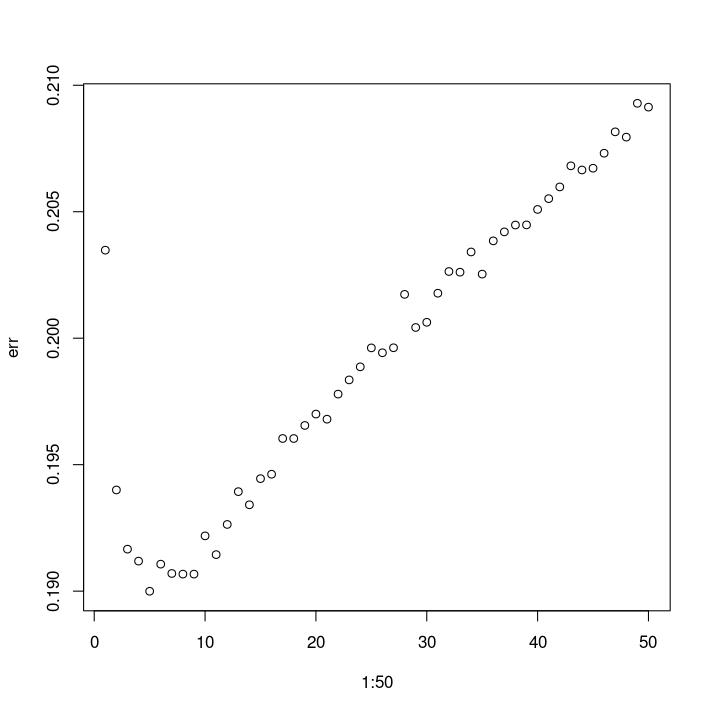
\includegraphics[scale=0.5]{mink}
    \end{center}
    \inputminted[linenos,frame=lines,framesep=2mm]{R}{knn.R}

    \subsection*{LDA}
    I had issues running hzTest on the entire data set with size of 19200, but I was 
    able to run it on a random subset of size 15000.
    So instead I resorted to running it on a random subset of the data. \\
    Both the hzTest and uniPlot indicated that the data was not multi-variate norm.
    From the plot we can see that some features look almost normal, but overall the data
    does not follow a normal distribution. Because of this, we can expect LDA and QDA to
    not perform particularly well. \\
    Running these methods anyway produced the expected results both performed at about 
    78\% accuracy on test, which is less than I was able to achieve with KNN. \\
    \bigbreak
    \inputminted[frame=lines,framesep=2mm]{text}{norm.txt}
    \bigbreak
    \begin{center}
	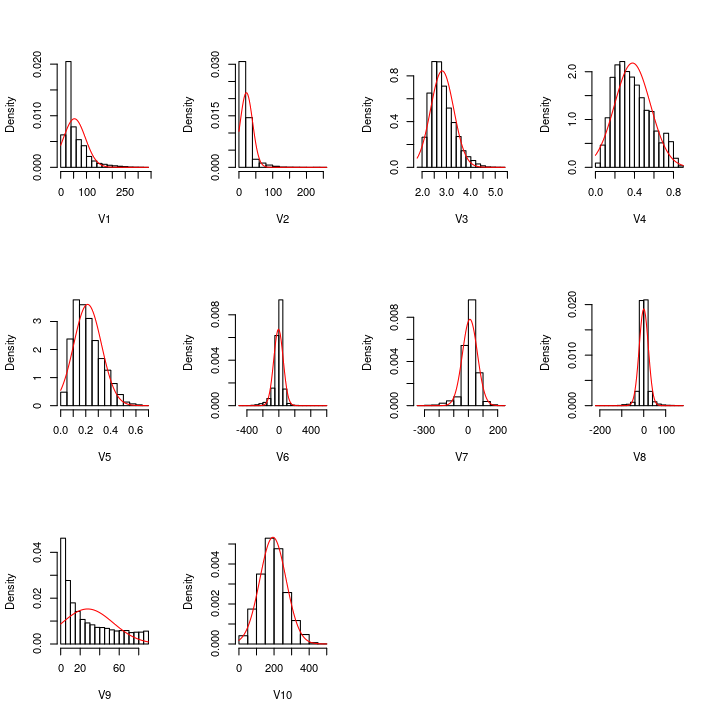
\includegraphics[scale=0.5]{hist}
    \end{center}
    \inputminted[linenos,frame=lines,framesep=2mm]{R}{lda.R}

    \subsection*{QDA}
    Due to the poor performance of LDA, and the non-linear nature of the input data set,
    we do not expect QDA to perform any better.
    It may have one assumption less than LDA, the assumption it keeps still fails.
    Running the algorithm produces a mean accuracy roughly equivalent to that 
    produced by LDA. \\
    \inputminted[linenos,frame=lines,framesep=2mm]{R}{qda.R}

    \subsection*{Naive Bayes (Normal)}
    Naive Bayes was less interesting, again, as was the case with LDA, the normal 
    assumption of the data set failed, but I went ahead and ran it anyway.
    The results were unexciting, serving as the worst performing classifier
    over 100 random test cases. \\
    \inputminted[linenos,frame=lines,framesep=2mm]{R}{bayes_norm.R}

    \subsection*{Naive Bayes (Kernel)}
    Removing the normal assumption of the input data set increased the processing time
    required to train a model using Naive Bayes with a Kernel density estimation. But
    this resulted in an improvement in accuracy over Naive Bayes with a Normal assumption.
    Despite this it still performed worse than LDA and QDA, much less KNN. \\
    \inputminted[linenos,frame=lines,framesep=2mm]{R}{bayes_kern.R}

\problem{}

\begin{enumerate}
    \item Classify the test point (0, 1) using QDA and calculate 
	the posterior class probabilities. Do the calculations by hand.
    \item Classify the test point (0, 1) using naive Bayes assuming 
	normality and calculate the posterior class probabilities.
	Do the calculations by hand.
    \item Verify your results for both classifiers using Matlab, R, etc.
	You can use the built-in functions.

\end{enumerate}

\solution

\part
    First we need to calculate the class means $\Hat{\mu}_0$ and $\Hat{\mu}_1$ \\
    \begin{align*}
	\Hat{\mu}_0 &= \frac{1}{3} ([0.6585,0.2444] + [2.2460,0.5281] + [-2.7665,-3.8303]) &\\
	    &= \frac{1}{3} [0.138, -3.8303]\ &\\
	    &= [0.046, -1.019267] &\\
	\Hat{\mu}_1 &= \frac{1}{3} ([-1.2565, 3.4912] + [-0.7973, 1.2288] + [1.1170, 2.2637]) &\\
	    &= \frac{1}{3} [-0.9368, 6.9837]\ &\\
	    &= [-0.3122667, 2.3279000] &\\
    \end{align*}

    Next calculate the covariance matrix for each class.

    \begin{align*}
	\Hat{\Sigma}_0 &= \frac{1}{2}(
	    ([0.6585, 0.2444] - \Hat{\mu}_0)([0.6585, 0.2444] - \Hat{\mu}_0)^\intercal &\\
	    &+ ([2.2460, 0.5281] - \Hat{\mu}_0)([2.2460, 0.5281] - \Hat{\mu}_0)^\intercal &\\
	    &+ ([-2.7665, -3.8303] - \Hat{\mu}_0)([-2.7665, -3.8303] - \Hat{\mu}_0)^\intercal &\\
	    &= 
		\frac{1}{2} (
		    \begin{bmatrix}
			0.33516 & 0.77400 \\
			0.77400 & 1.59685 \\
		    \end{bmatrix}
		    +
		    \begin{bmatrix}
			4.8400 & 3.4042 \\
			3.4042 & 2.394
		    \end{bmatrix}
		    +
		    \begin{bmatrix}
			7.9102 & 7.9060 \\
			7.9060 & 7.9019 \\
		    \end{bmatrix}
		) &\\
	    &=
		\begin{bmatrix}
		    6.5627 & 6.0421 \\
		    6.0421 & 5.9466
		\end{bmatrix}
    \end{align*}

    \begin{align*}
	\Hat{\Sigma}_1 &= \frac{1}{2}(
	    ([-1.2565, 3.4912] - \Hat{\mu}_1)([-1.2565, 3.4912] - \Hat{\mu}_1)^\intercal &\\
	    &+ ([-0.7973, 1.2288] - \Hat{\mu}_1)([-0.7973, 1.2288] - \Hat{\mu}_1)^\intercal &\\
	    &+ ([1.1170, 2.2637] - \Hat{\mu}_1)([1.1170, 2.2637] - \Hat{\mu}_1)^\intercal &\\
	    &= 
		\frac{1}{2} (
		    \begin{bmatrix}
			0.89158 & -1.09843 \\
			-1.09843 & 1.35327
		    \end{bmatrix}
		    +
		    \begin{bmatrix}
			0.23526 & 0.53310 \\
			0.53310 & 1.20802 
		    \end{bmatrix}
		    +
		    \begin{bmatrix}
			2.0426033 & -0.0917589 \\
			-0.0917589 & 2.0426033
		    \end{bmatrix}
		) &\\
	    &=
		\begin{bmatrix}
		    1.58482 & -0.32854 \\
		    -0.32854 & 1.28270 
		\end{bmatrix}
    \end{align*}

    \bigbreak
    We would like to maximize $\Hat{P}[Y=k]\hspace{1pt}\Hat{f}(X=x|Y=k)$ 
	over $k\in\{0,1\}$ for our input x=(0,1).

    $$
	\argmax_{k\in\{0,1\}} 
	\Hat{P}[Y=k]
	\biggr(\frac{1}{(2\pi)^{\frac{d}{2}}{|\Hat{\Sigma}_k}|^{\frac{1}{2}}}\biggr)
	\exp(\frac{1}{2}(x - \Hat{\mu}_k)^\intercal \Hat{\Sigma}_k^{-1} (x - \Hat{\mu}_k))
    $$

    \textbf{case: k = 0} \\

    \begin{align*}
	\Hat{P}[Y=0] = \frac{3}{6} &= \frac{1}{2} &\\
	|\Hat{\Sigma}_0| = 2.5180 \Rightarrow |\Hat{\Sigma}_0|^{\frac{1}{2}} &= 1.5868 &\\
	\biggr(\frac{1}{(2\pi)^{\frac{2}{2}}{|\Hat{\Sigma}_0}|^{\frac{1}{2}}}\biggr) =
	    (\frac{1}{9.9702}) &= 0.10030 &\\
	\exp(\frac{1}{2}(x - \Hat{\mu}_0)^\intercal \Hat{\Sigma}_0^{-1} (x - \Hat{\mu}_0)) &=  &\\
	    \exp(-\frac{1}{2} * 11.078) = \exp(-5.5389) &= 0.0039308 &\\
	\Hat{P}[Y=0]\hspace{1pt}\Hat{f}(X=x|Y=0) &= .00019713
    \end{align*}

    \textbf{case: k = 1} \\

    \begin{align*}
	\Hat{P}[Y=1] = \frac{3}{6} &= \frac{1}{2} &\\
	|\Hat{\Sigma}_1| = 1.9249 \Rightarrow |\Hat{\Sigma}_1|^{\frac{1}{2}} &= 1.3874 &\\
	\biggr(\frac{1}{(2\pi)^{\frac{2}{2}}{|\Hat{\Sigma}_1}|^{\frac{1}{2}}}\biggr) =
	    \frac{1}{8.7174} &= 0.11471 &\\
	\exp(-\frac{1}{2}(x - \Hat{\mu}_1)^\intercal \Hat{\Sigma}_1^{-1} (x - \Hat{\mu}_1)) &= &\\
	    \exp(-\frac{1}{2} * 1.3752) = \exp(-0.6876) &= 0.50278 &\\
	\Hat{P}[Y=1]\hspace{1pt}\Hat{f}(X=x|Y=1) &= 0.028838
    \end{align*}

    \clearpage
    Noting that $0.00019713 < 0.028838$, k=1 maximizes our function, thus we 
    predict a class label of 1 for (0,1).
    The posterior class probability is given by the following function.

    \begin{align*}
	P[Y=k|X=x] &= \frac{P[Y=k]f_{1\ldots d}(X=x|Y=k)}
	    {\sum_{i=0}^{k} P[Y=i]f_{Y\ldots d}(X=x|Y=i)} &\\
	&= \frac {0.028838} {0.028838 + 0.00019713} &\\
	&= 0.99321
    \end{align*}

    Thus we find that we have a posterior class probability of $99.321\%$ for class k=1.

\part

    The naive Bayes classification uses the same class norms $\Hat{\mu}_0$ and $\Hat{\mu}_1$. \\
    However we will need to compute $\Hat{\sigma}^2$ values for each feature of each class. \\

    \bigbreak
    \textbf{case: k = 0} \\

    First compute the variance of each feature.

    \begin{align*}
	\Hat{\sigma}_0^2 &= \frac{1}{3} * \sum_{j\in C_0} (x_i - \Hat{\mu}_i)^2 &\\
	&= \frac{1}{3}(
	    ((0.6585, 0.2444) - \Hat{\mu}_0)^2 
	    + ((2.2460, 0.5281) - \Hat{\mu}_0)^2 
	    + ((-2.7665, -3.8303) - \Hat{\mu}_0)^2) &\\
	&= \frac{1}{3}(13.125, 11.893) &\\
	&= (4.3751, 3.9644) &\\
    \end{align*}

    Now we can compute $f_i((0,1)|Y=0)$ for use in our classifier.

    \begin{align*}
	f((0,1)|Y=0) &= \frac{1}{\sqrt{2\pi\Hat{\sigma}_0^2}}
	    e^{-\frac{(<0,1>-\Hat{\mu}_0)^2}{2\Hat{\sigma}_0^2}} &\\
	&= \frac{1}{(5.2431, 4.9909)} (0.99976, 0.59794) &\\
	&= (0.19068, 0.11981)
    \end{align*}

    We would like to maximize the following equation over all k
    $ \Hat{P}[Y=0]\prod_{i=1}^{d}f_i(X_i|Y=k) $. \\

    \begin{align*}
	\Hat{P}[Y=0] &= \frac{3}{6} &\\
	f_0(X_0|Y=0) &= 0.19068 &\\
	f_1(X_1|Y=0) &= 0.11981 &\\
	\frac{1}{2}*0.19068*0.11981 &= 0.011423
    \end{align*}

    \bigbreak
    \textbf{case: k = 1} \\

    First compute the variance of each feature.

    \begin{align*}
	\Hat{\sigma}_1^2 &= \frac{1}{3} * \sum_{j\in C_1} (x_i - \Hat{\mu}_i)^2 &\\
	&= \frac{1}{3}(((-1.2565, 3.4912) - \Hat{\mu}_1) ^2 
	    + ((-0.7973, 1.2288) - \Hat{\mu}_1)^2 + (1.1170, 2.2637) - \Hat{\mu}_1)^2) &\\
	&= \frac{1}{3}(3.1696, 2.5654) &\\
	&= (1.05655, 0.85514) &\\
    \end{align*}

    Now we can compute $f_i((0,1)|Y=1)$ for use in our classifier.

    \begin{align*}
	f((0,1)|Y=1) &= \frac{1}{\sqrt{2\pi\Hat{\sigma}_1^2}}
	    e^{-\frac{(<0,1>-\Hat{\mu}_1)^2}{2\Hat{\sigma}_1^2}} &\\
	&= \frac{1}{(2.5765, 2.3180)} (0.95490, 0.35664) &\\
	&= (0.37062, 0.15386)
    \end{align*}

    We would like to maximize the following equation over all k
    $\Hat{P}[Y=1]\prod_{i=1}^{d}f_i(X_i|Y=k)$.

    \begin{align*}
	\Hat{P}[Y=1] &= \frac{3}{6} &\\
	f_0(X_0|Y=0) &= 0.37062 &\\
	f_1(X_1|Y=0) &= 0.15386 &\\
	\frac{1}{2}*0.37062*0.15386 &= 0.028512
    \end{align*}

    Noting that $0.011423 < 0.028512$, k=1 maximizes our function, thus we 
    predict a class label of 1 for (0,1).
    The posterior class probability is given by the following function.

    \begin{align*}
	P[Y=k|X=x] &= \frac{P[Y=k]f_{1\ldots d}(X=x|Y=k)}
	    {\sum_{i=0}^{k} P[Y=i]f_{Y\ldots d}(X=x|Y=i)} &\\
	&= \frac {0.028512} {0.028512 + 0.011423} &\\
	&= 0.71396
    \end{align*}

    Thus we find that we have a posterior class probability of $71.396\%$ for class k=1.

\part

    I have included the results of the R script that follows as comments directly
    below the corresponding print statements. The result of qda(\ldots) in R
    produces the exact same posterior class probability as I have computed above.
    Currently my results for NaiveBayes(\ldots) are off by about 4\%, so I must
    have an error in my work somewhere.
    \inputminted[linenos,frame=lines,framesep=2mm]{R}{p2.R}

\end{document}
